\section[The course]{The LIKE Open Science Course}
\stepcounter{subsection} %We don't use subsection titles, only frametitles
\label{sec:course}

%---------------------------------------------------------------
% 1. What is open science?
%---------------------------------------------------------------
\begin{frame}{What is this ``Open Science'' thing anyway?}

\begin{quotation}<1->
Open science is the movement to make scientific research and its dissemination accessible to all levels of an inquiring society, amateur or professional. \\
Open science is transparent and accessible knowledge that is shared and developed through collaborative networks.
\begin{flushright}
    \tiny{---\textlink{https://en.wikipedia.org/wiki/Open_science}{Wikipedia}}
  \end{flushright}
\end{quotation}

\begin{columns}
    \begin{column}{.45\textwidth}
    % it is...
        \begin{block}<2->{It is...}
            \begin{itemize}
                \item A philosophy
                \item A set of tools
                \item An old idea
            \end{itemize}
        \end{block}
    \end{column}
    
    \begin{column}{.45\textwidth}
    % it is not...
        \begin{block}<2->{It is not...}
            \begin{itemize}
                \item Difficult
                \item Expensive
                \item Rewarded directly
            \end{itemize}
        \end{block}
    \end{column}
    
\end{columns}

\end{frame}


%---------------------------------------------------------------
% 2. High-level goals
%---------------------------------------------------------------

% high-level goals
\begin{frame}{Course goals}

\begin{columns}[t]
    % LHS text
    \begin{column}{.45\textwidth}

    \textbf{We want you to be successful.}
    \vspace{3ex}
    

    This course will:
    \begin{itemize}
        \item Tell you about open science
        \item Give you a toolbox
        \item Help you use these tools
    \end{itemize}
    
    \end{column}

    % RHS image
    \begin{column}{.45\textwidth}

        \centering
        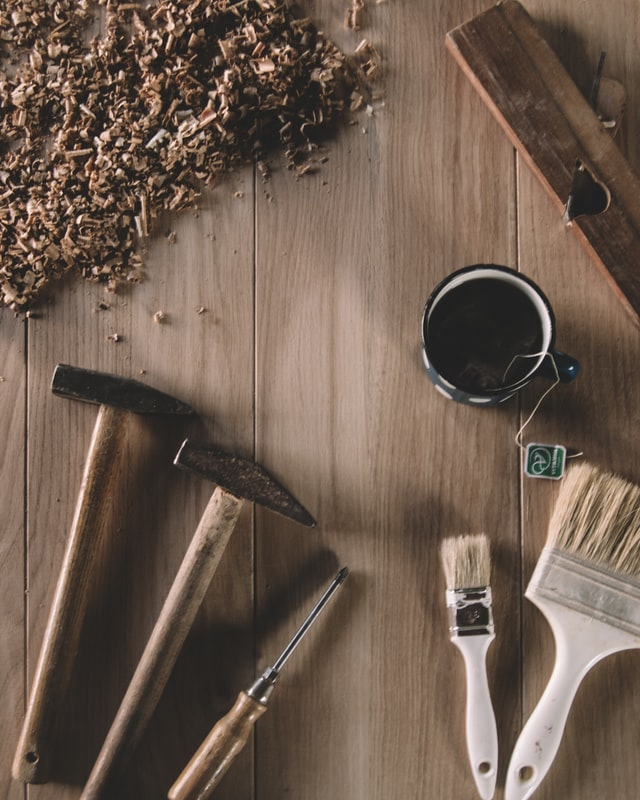
\includegraphics[width=0.8\textwidth]{images/milan-popovic-BmyXTxyDL-I-unsplash.jpg}
    
        \givecredit{\centering Photo by \textlink{https://unsplash.com/@itsmiki5?utm_source=unsplash&amp;utm_medium=referral&amp;utm_content=creditCopyText}{Milan Popovic} on \textlink{https://unsplash.com/s/photos/tools?utm_source=unsplash&amp;utm_medium=referral&amp;utm_content=creditCopyText}{Unsplash}}
    
    \end{column}

\end{columns}


\end{frame}

%---------------------------------------------------------------
% 3. Calendar
%---------------------------------------------------------------

\begin{frame}{Course outline}

\begingroup
\renewcommand{\arraystretch}{0.9} % Default value: 1
\setlength\tabcolsep{0pt}  % default value: 6pt
% Table based on https://github.com/LIKE-ITN/OpenScienceTrainingCourse/blob/master/readme.md#course-outline
\setlength{\fboxsep}{3pt}
\colorbox{uniSgray!10}{%

    \begin{tabular}{@{}p{0.35\textwidth}p{0.35\textwidth}p{0.3\textwidth}@{}}
        Seminar & Self study & Deliverable \\ 
        \midrule
        1. \textlink{https://github.com/LIKE-ITN/OpenScienceTrainingCourse/blob/master/seminar1/seminar1.md}{Introducing open science} &  &  \\ 
         &  1. \textlink{https://github.com/LIKE-ITN/OpenScienceTrainingCourse/blob/master/selfstudy1.md}{Background reading} &  \\ 
        2. \textlink{https://github.com/LIKE-ITN/OpenScienceTrainingCourse/blob/master/seminar2.md}{Guiding principles} &  &  \\ 
         & 2. \textlink{https://github.com/LIKE-ITN/OpenScienceTrainingCourse/blob/master/selfstudy2.md}{Is your group's work FAIR?} &  \\ 
        3. \textlink{https://github.com/LIKE-ITN/OpenScienceTrainingCourse/blob/master/seminar3.md}{Open science and intellectual property} &  &  \\ 
         & 3. \textlink{https://github.com/LIKE-ITN/OpenScienceTrainingCourse/blob/master/selfstudy3.md}{Implementing open science} & \\ 
        4. \textlink{https://github.com/LIKE-ITN/OpenScienceTrainingCourse/blob/master/seminar3.md}{Communicating your science} &  &  \\ 
         & 4. \textlink{https://github.com/LIKE-ITN/OpenScienceTrainingCourse/blob/master/selfstudy4.md}{Communications strategies} &  \\ 
         &  & 1. \textlink{https://github.com/LIKE-ITN/OpenScienceTrainingCourse/blob/master/deliverable1.md}{Implementation case study} \\ 
         5. \textlink{https://github.com/LIKE-ITN/OpenScienceTrainingCourse/blob/master/seminar5.md}{What are data management plans and why do they matter?} &  &   \\ 
         & 5. \textlink{https://github.com/LIKE-ITN/OpenScienceTrainingCourse/blob/master/selfstudy5.md}{Draft a data management plan} &  \\ 
        Workshop: \textlink{https://github.com/LIKE-ITN/OpenScienceTrainingCourse/blob/master/workshop1.md}{Open science in LIKE} &  & \\ 
         & 6. \textlink{https://github.com/LIKE-ITN/OpenScienceTrainingCourse/blob/master/selfstudy6.md}{Revise data management plan} &  \\ 
         &  & 2. \textlink{https://github.com/LIKE-ITN/OpenScienceTrainingCourse/blob/master/deliverable2.md}{Data management plan} \\ 
         
    \end{tabular}
}\endgroup

\end{frame}

%---------------------------------------------------------------
% 3. Logistics - Office Hours, Questions, Etc.
%---------------------------------------------------------------

\begin{frame}{Course logistics}
    
    \begin{columns}
    \column{.45\textwidth}
   
        \begin{block}{Grading}
            \begin{itemize}
                \item No exams, but..
                \item Deliverables needed for a participation certificate. 
            \end{itemize}
        \end{block}

        \begin{block}{Questions?}
            \begin{itemize}
                \item No office hours!
                \item Use slack and ask each other
            \end{itemize}
        \end{block}

    \column{.45\textwidth}
    
        \begin{block}{Errors, suggestions, corrections...}
            \begin{itemize}
                \item  \textlink{https://github.com/LIKE-ITN/OpenScienceTrainingCourse/issues}{Help improve the material} 
            \end{itemize}
        \end{block}

        \begin{block}{Your feedback}
        This is a new course!
            \begin{itemize}
                \item Get in touch at any time
                \item Survey at the end
            \end{itemize}
        \end{block}

        \end{columns}
    
\end{frame}
